\documentclass[11pt, twocolumn]{article}

\usepackage[english]{babel}
\usepackage{graphicx}
\usepackage{imakeidx}
\usepackage{mathrsfs, amsmath}
\usepackage{systeme}
\usepackage{array}
\usepackage[utf8]{inputenc}
\usepackage{siunitx}
\usepackage{booktabs}
\usepackage{adjustbox}
\usepackage{geometry}
\geometry{a4paper,total={150mm,215mm}}
\usepackage{makecell}
\usepackage{afterpage}
\usepackage{listings}
\usepackage{subcaption}
\usepackage[toc,page]{appendix}
\usepackage[table]{xcolor}
\usepackage{pifont} % ding symbols
\usepackage{tikz}
\usepackage{changepage}
\usepackage{multirow} % multi row in tables
\usepackage{booktabs}
\usepackage{textcomp} % registered and copyright symbol
\usepackage{lscape} % vertical instead to horizontal 
\usepackage{longtable} % for more page tables
\usepackage{eurosym}
\usepackage{lmodern}
\usepackage{amstext}
\usepackage{pdfpages} % import pdf pages
%\usepackage[hidelinks]{hyperref} % delete ugly hyperref borders of hyperlink
\usepackage{hyperref} % internal hyperlinks
\usepackage{titling} % titles
\usepackage{blindtext} % for casual texts
\usepackage{dblfloatfix} % forces image at bottom in two-column files

\DeclareRobustCommand{\officialeuro}{%
  \ifmmode\expandafter\text\fi
  {\fontencoding{U}\fontfamily{eurosym}\selectfont e}}



\makeindex[columns=2, title=Indice alfabetico, options= -s mystyle.ist, intoc]

\newcommand*{\Scale}[2][4]{\scalebox{#1}{\ensuremath{#2}}}
\renewcommand*\contentsname{Indice}
\newcommand*\NewPage{\newpage\null\thispagestyle{empty}\newpage}
\newcommand{\Virgolette}[1]{``#1''}
\newcommand*\circled[1]{\tikz[baseline=(char.base)]{
	\node[shape=circle,draw,inner sep=2pt] (char) {#1};}}
\newcommand{\tikzcircle}[2][red,fill=red]{\tikz[baseline=-0.5ex]\draw[#1,radius=#2] (0,0) circle ;}%command for draw text circle coloured
\def\changemargin#1#2{\list{}{\rightmargin#2\leftmargin#1}\item[]}
\let\endchangemargin=\endlist
\makeatletter
\let\originalpart=\part


            
\newcolumntype{C}[1]{>{\centering\arraybackslash}p{#1}}
\newcolumntype{L}[1]{>{\arraybackslash}p{#1}}
\newcolumntype{R}[1]{>{\raggedleft}p{#1}}
\newcolumntype{G}[1]{>{\centering\arraybackslash\columncolor{gray0}}p{#1}}

\definecolor{gray0}{gray}{0.9}
\definecolor{gray1}{gray}{0.7}
\definecolor{gray2}{gray}{0.4}

\lstset{
	literate = {α}{{$\alpha$}}1 {∆}{{$\Delta$}}1 {θ}{{$\theta$}}1 {η}{{$\eta$}}1 {→}{{$\rightarrow$}}1 {∂}{{$\partial$}}1, %tutti i simboli da usare come codice
	language = Mathematica % linguaggio
}
\hypersetup{
	citebordercolor=red
}


% ----- TITLE
\title{
	\large{University of Trento}\\
	\normalsize{Depertment of Industrial Engineering}\\
	\normalsize{Master in Mechatronics Engineering}\\
	\vspace{0.5cm}
	\Large{\textit{Modelling and simulation of mechatronic systems}}\\
	\vspace{0.2cm}
	\huge{\textbf{Development, analysis and optimization of the performance of an innovative driving simulator}}\\
	\vspace{0.25cm}
	\hrule
	\vspace{0.2cm}
	\Large{\textbf{System requirements}}\\	% Title
	\vspace{0.2cm}
	\hrule
}
\author{A. Comoretto \and J. Losi \and S. Valentini}
\date{}
% ----- TITLE


\begin{document}
\maketitle
The objective of this project is to develope, analyze and optimize the performance of an innovative driving simulator.
A simulator is a device that enables the operator to reproduce or represent under test conditions phenomena likely to occur in actual performance.
Driving simulators are in general used both for research purposes and in the development process of a vehicle.

The simulator has to emulate the behaviour of a car like the one shown in Figure \ref{f:RefereeSystem}.
\begin{figure}[h!]
	\centering
	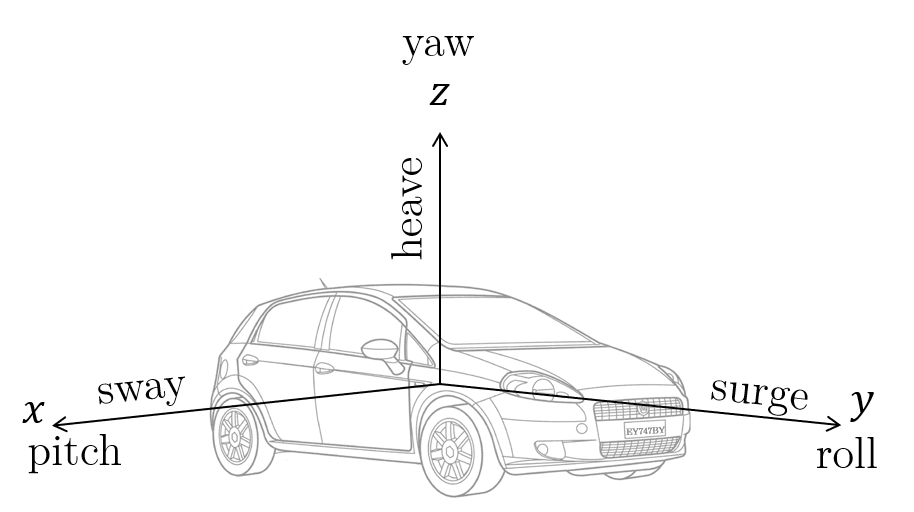
\includegraphics[width=7.5cm]{Images/Car_axes}
	\caption{Referee system used.}
	\label{f:RefereeSystem}
\end{figure}
In the first phase of the project it is relevant to impose a correct set of objective which are composed by system requirements, engineering specifications and performance indices.
To make the correct choice literature have been consulted and physical tests have been conduced.


\colorbox{yellow}{***}\\


\colorbox{yellow}{PARAMETRI E RELATIVE FONTI}\\
\colorbox{yellow}{catalogo}\\
\colorbox{yellow}{sperimentale}

\colorbox{yellow}{INDICI DI PERFORMANCE}\\
\colorbox{yellow}{cinematici}\\
\colorbox{orange}{dinamici}



\begin{figure}[h!]
	\centering
	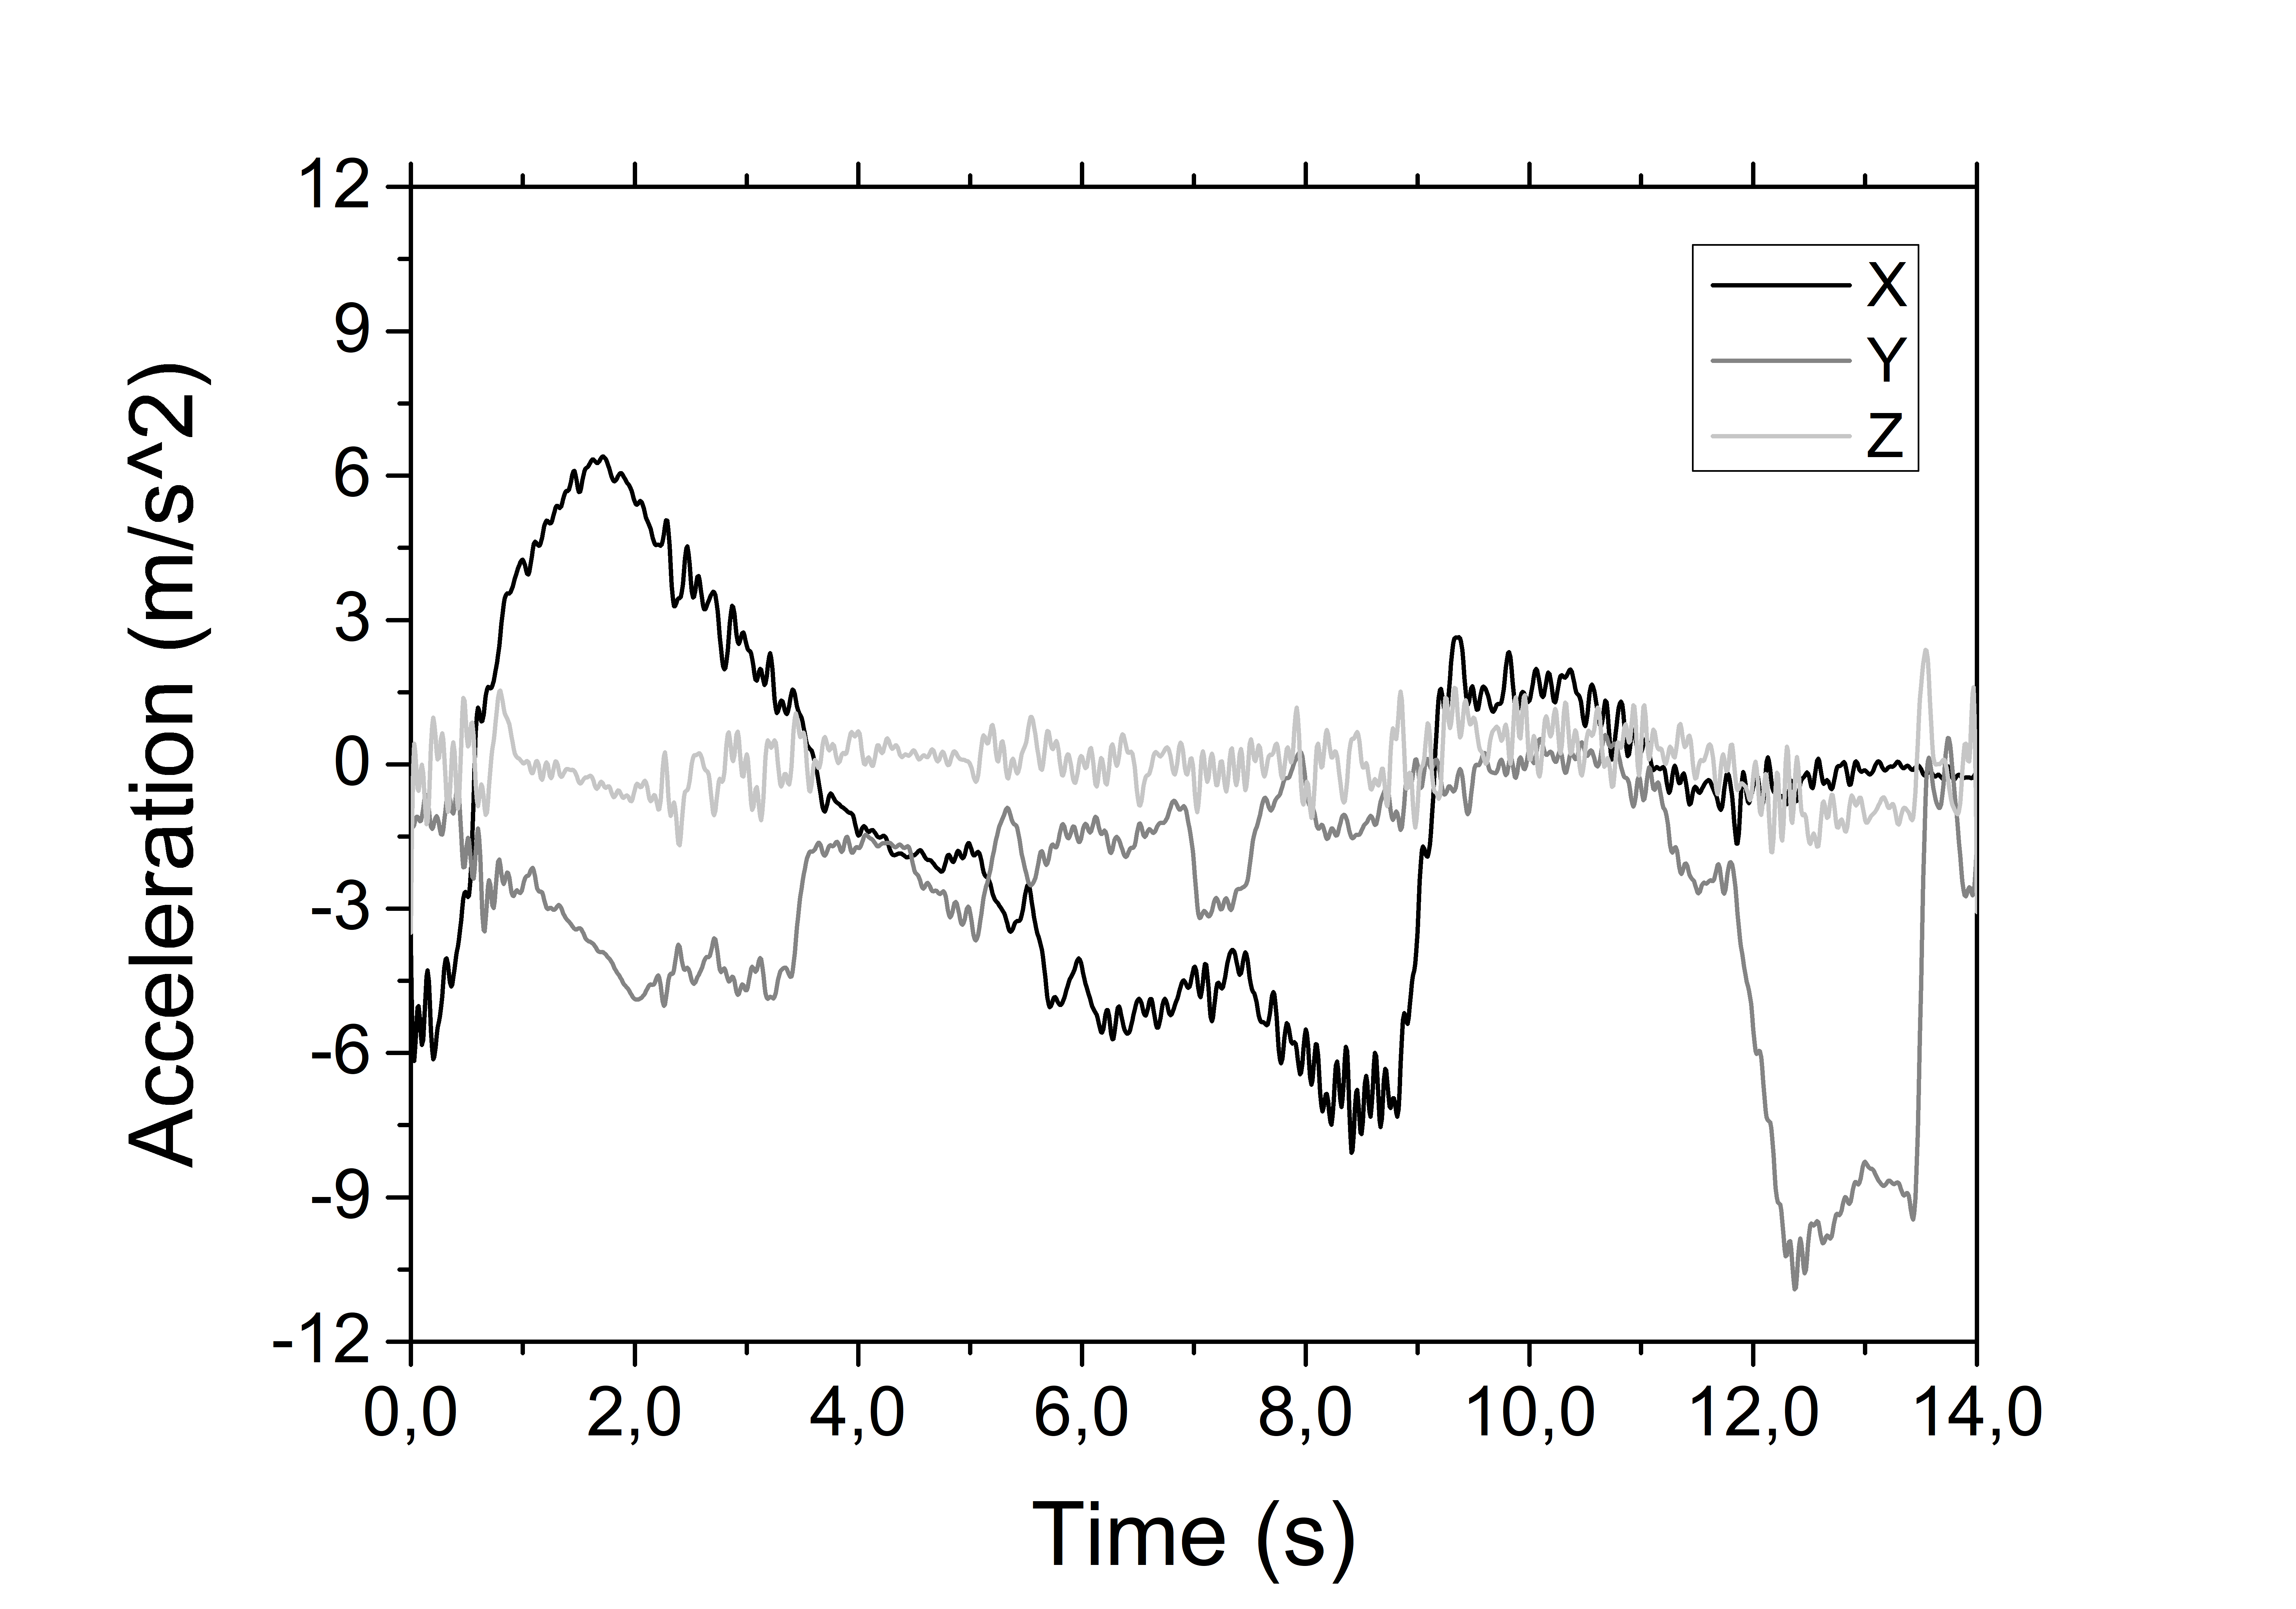
\includegraphics[width=8cm]{Images/Acceleration}
\end{figure}

\begin{figure}[h!]
	\centering
	\includegraphics[width=8cm]{Images/FFTStationary}
\end{figure}

\begin{figure}[h!]
	\centering
	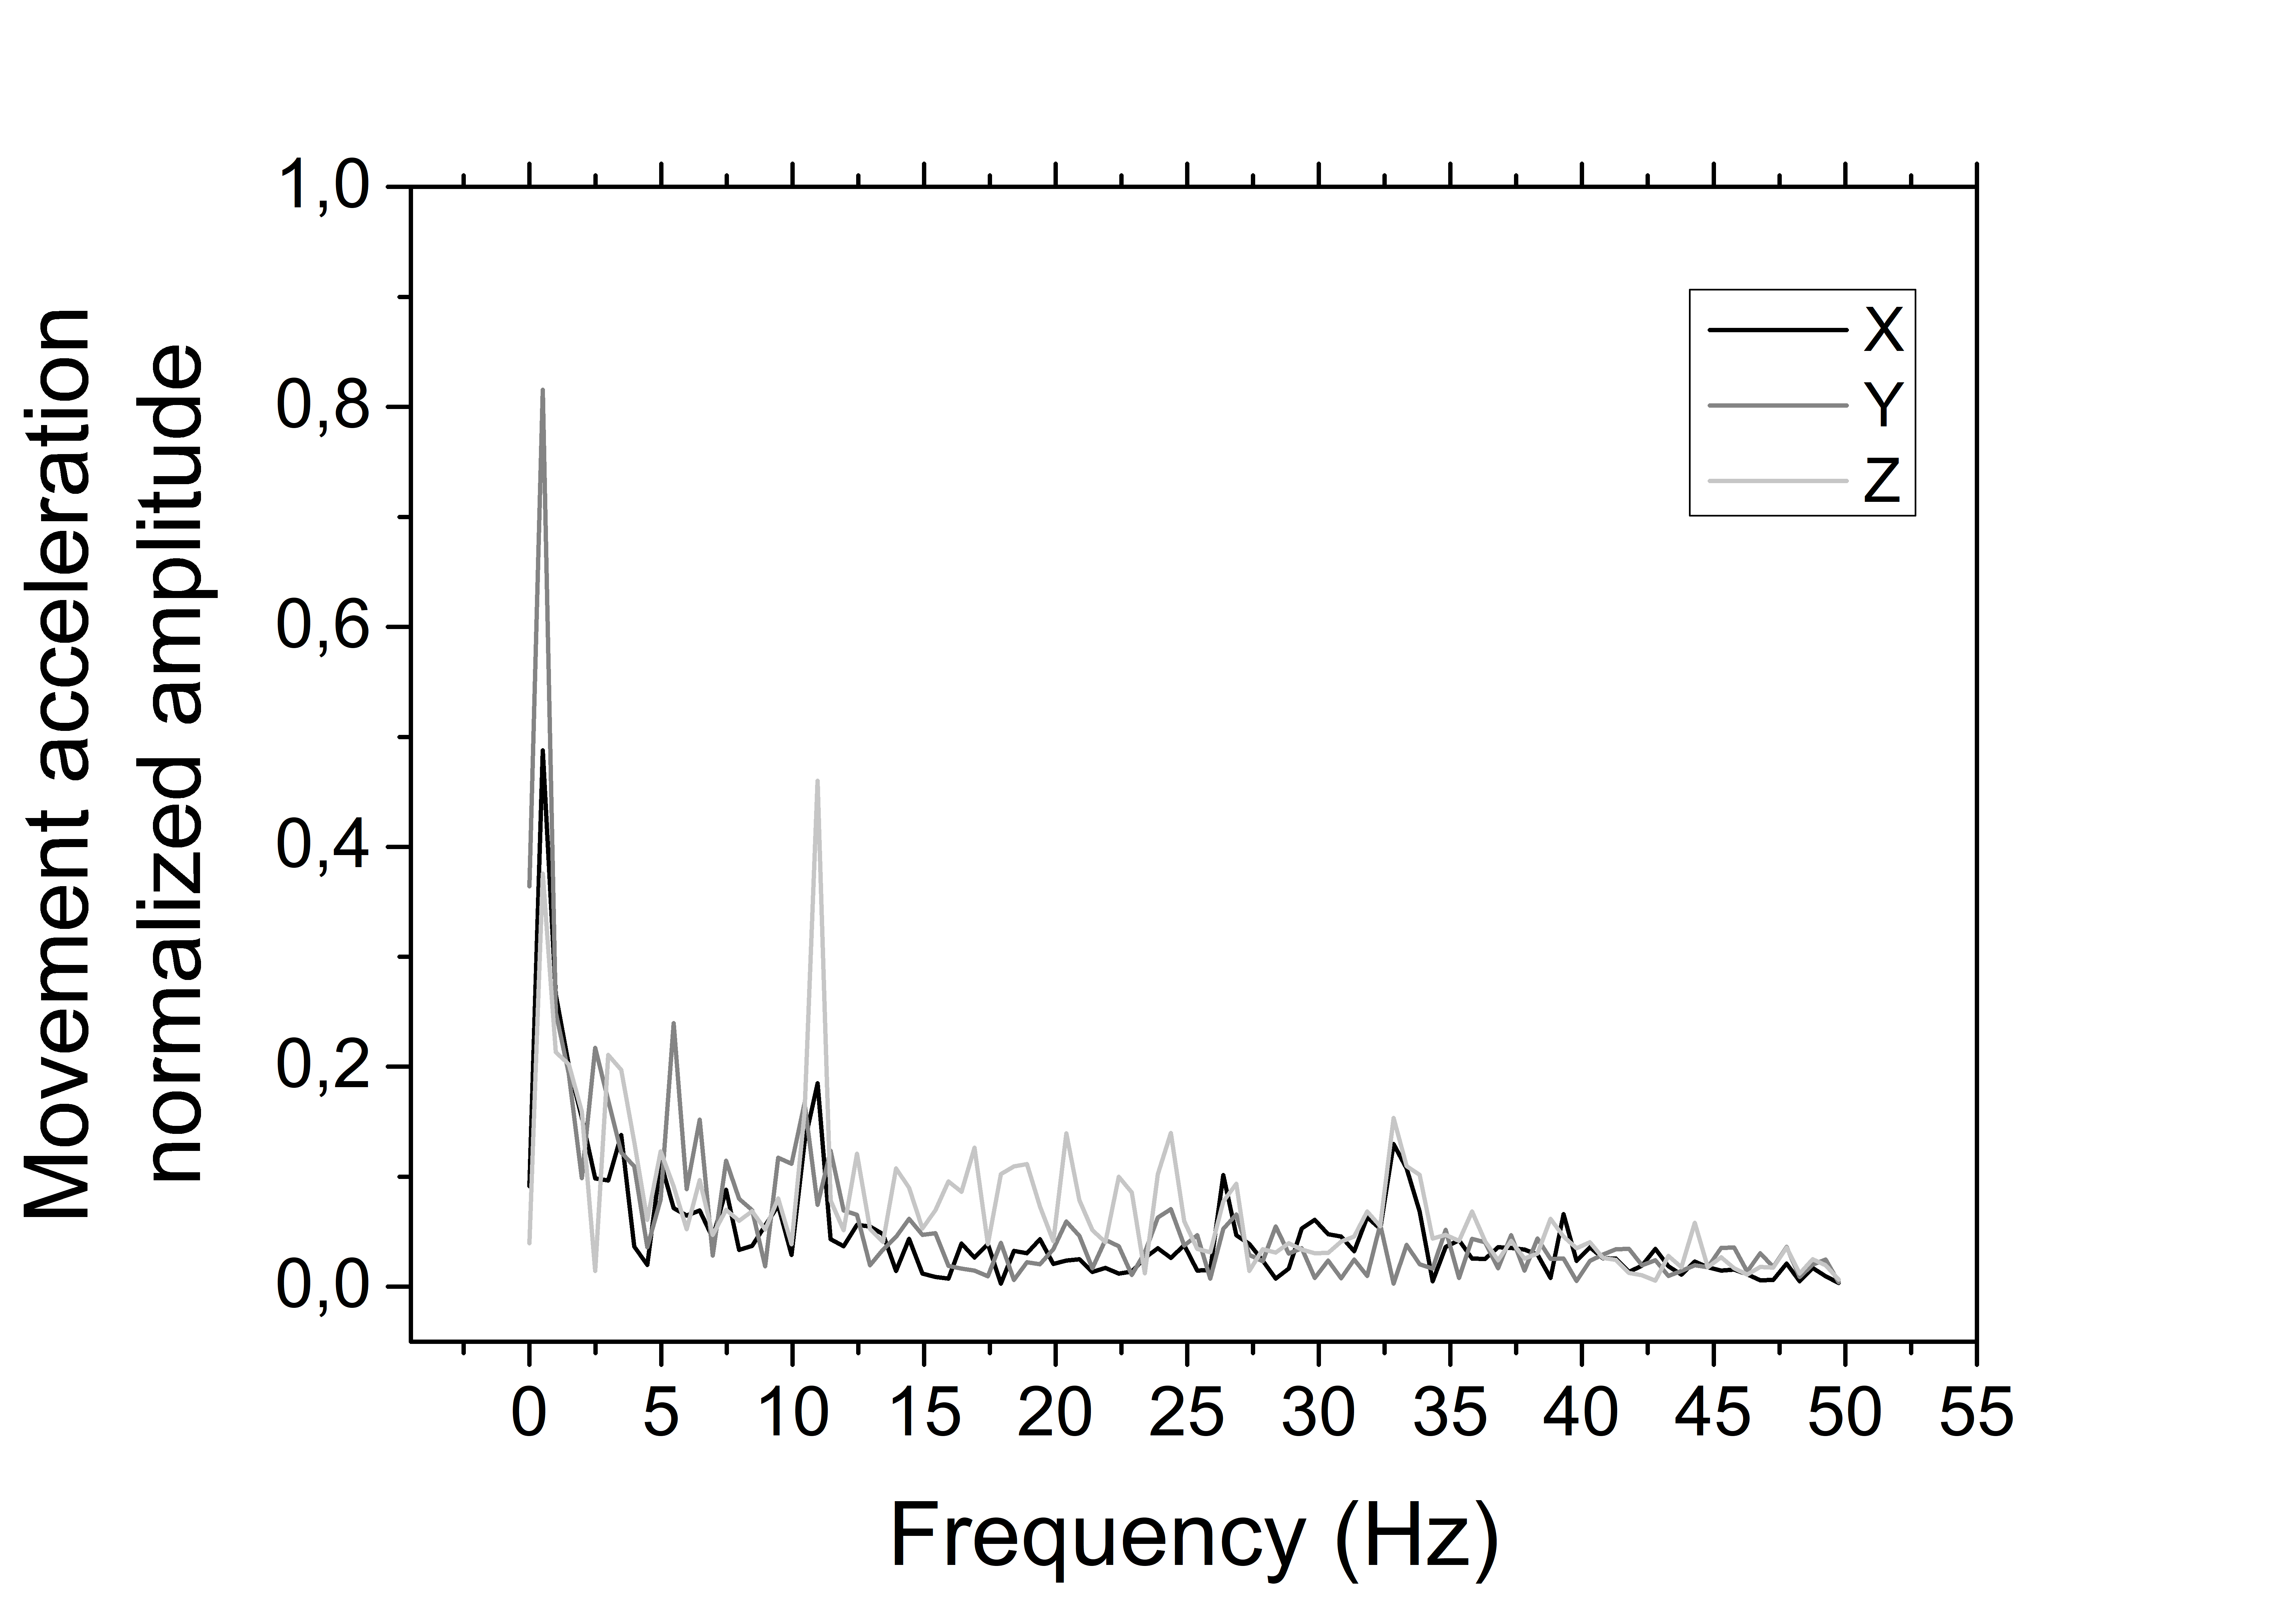
\includegraphics[width=8cm]{Images/FFTMovement}
\end{figure}


\begin{table*}[b]
\centering
\begin{changemargin}{-0.5cm}{-0.5cm}
\centering
\begin{tabular}{C{1.25cm}C{1.25cm}C{1.25cm}C{1.25cm}C{1.25cm}C{1.25cm}C{1.25cm}C{1.25cm}C{1.25cm}C{1.25cm}}
	\textbf{Yaw} & \textbf{Pitch} & \textbf{Roll} & \textbf{Surge} & \textbf{Sway} & \textbf{Heave} & \textbf{Length} & \textbf{Width} & \textbf{Payload}\\
	\hline
	\hline
	\\
	cell 1 & cell 2 & cell 3\\
	\\
	\hline
\end{tabular}
\end{changemargin}
\caption{System requirements.}
\label{t:SystemRequirements}
\end{table*}


\begin{thebibliography}{}
\bibitem{aVDS}
\Virgolette{\textit{Advanced Vehicle Driving Simulator}}, \textsc{ABDynamics}.

\bibitem{CKAS}
\Virgolette{\textit{6DOF Motion System}}, \textsc{CKAS}.

\bibitem{Kasim}
M. Kasim A. J., \Virgolette{\textit{Design and development of 6-dof motion platform for vehicle driving simulator}}, Universiti Teknologi Malaysia.
\end{thebibliography}
\end{document}
